\chapter{Project and Media Attributes}%
\label{cha:project_and_media_attributes}

When you play media files in Cinelerra, the media files have a certain number of tracks, frame size, sample size, and so on. No matter what attributes the media file has, it is played back according to the project attributes. So, if an audio file's sample rate is different than the project attributes, it is resampled. Similarly, if a video file's frame size is different than the project attributes, the video is composited on a black frame, either cropped or bordered with black.

The project attributes are adjusted in Settings $\rightarrow$ Set Format (figure~\ref{fig:set-format}) or can be created in File $\rightarrow$ New. When you adjust project settings in File $\rightarrow$ New, a new empty timeline is created. Every timeline created from this point on uses the same settings. When you adjust settings in Settings $\rightarrow$ Format, media on the timeline is left unchanged. But every timeline created from this point uses the same settings.

\begin{figure}[htpb]
	\centering
	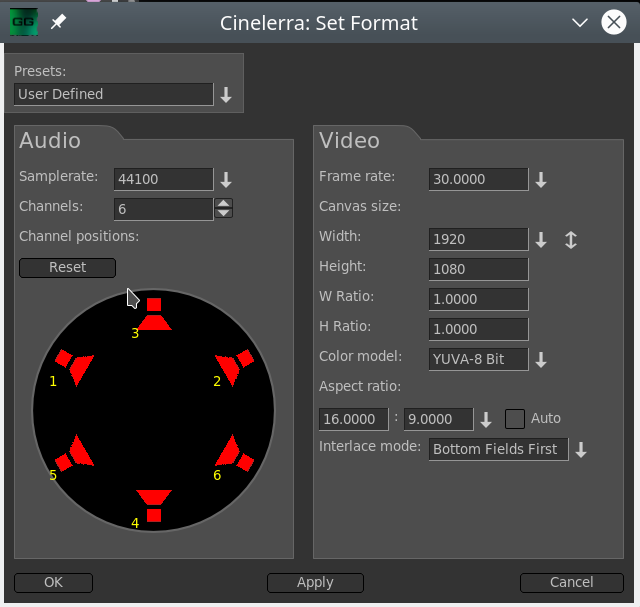
\includegraphics[width=0.5\linewidth]{images/set-format.png}
	\caption{Set Format window - note the Audio Channel positions}
	\label{fig:set-format}
\end{figure}

In addition to the standard settings for sample rate, frame rate, and frame size, Cinelerra uses some less traditional settings like channel positions, color model, and aspect ratio.  The aspect ratio refers to the screen aspect ratio.

Edit decision lists , the EDL stored in XML, save the project settings.  Formats which contain media but no edit decisions just add data to the tracks. Keep in mind details such as if your project sample rate is 48 kHz and you load a sound file with 96kHz, you will still be playing it at 48 kHz.  Or if you load an EDL file at 96kHz and the current project sample rate is 48 kHz, you will change it to 96 kHz.

The New Project window has some options that are different than the Set Format window as you can see by comparing figure~\ref{fig:set-format} above with this figure~\ref{fig:new-project}. Mostly notably is the field for a directory path and a Project Name.

\begin{figure}[htpb]
	\centering
	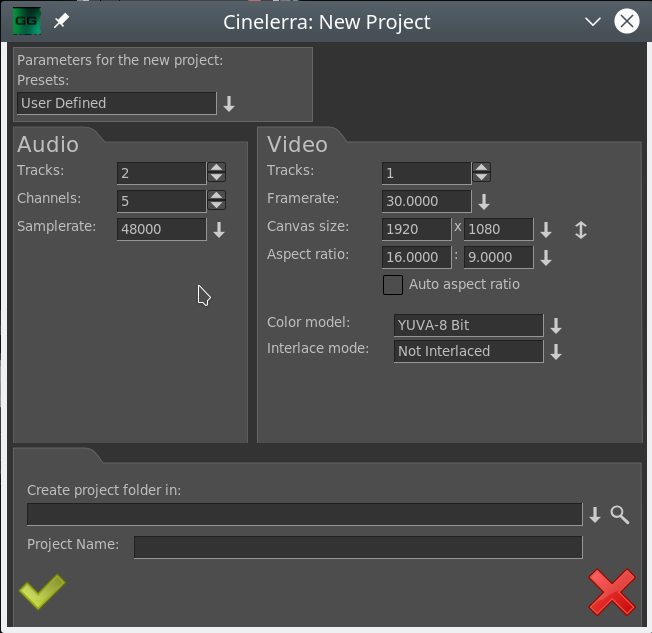
\includegraphics[width=0.5\linewidth]{images/new-project.png}
	\caption{New Project dialog window}
	\label{fig:new-project}
\end{figure}

Explanation of the various fields is described next.

\section{Audio attributes}%
\label{sec:audio_attributes}

\textit{Presets:}\\
select an option from this menu to have all the project settings set to one of the known standards.  Some of the options are 1080P/24, 1080I, 720P/60, PAL, NTSC, YouTube, and CD audio.

\textit{Tracks:}\\
(in New Project menu only) sets the number of audio tracks for the new project. Tracks can be added or deleted later, but this option is on the New Project menu for convenience.

\textit{Samplerate:}\\
sets the samplerate of the audio. The project samplerate does not have to be the same as the media sample rate that you load. Media is resampled to match the project sample rate.

\textit{Channels:}\\
sets the number of audio channels for the new project. The number of audio channels does not have to be the same as the number of tracks.

\textit{Channel positions:}\\
the currently enabled audio channels and their positions in the audio panning boxes in the track patchbay are displayed in the channel position widget in the Set Format window.  You can see this display on the left side in figure~\ref{fig:set-format} above. Channel positions are not in New Project window.

\vspace{1ex}The channels are numbered. When rendered, the output from channel 1 is rendered to the first output track in the file or the first sound card channel of the sound card. Later channels are rendered to output tracks numbered consecutively. The audio channel positions correspond to where in the panning widgets each of the audio outputs is located. The closer the panning position is to one of the audio outputs, the more signal that speaker gets. Click on a speaker icon and drag to change the audio channel location. The speakers can be in any orientation. A different speaker arrangement is stored for every
number of audio channels since normally you do not want the same speaker arrangement for different numbers of channels.

Channel positions is the only setting that does not affect the output necessarily. It is merely a convenience, so that when more than two channels are used, the pan controls on the timeline can distinguish between them. It has nothing to do with the actual arrangement of speakers. Different channels can be positioned very close together to make them have the same output.

\section{Video attributes}%
\label{sec:video_attributes}

\textit{Tracks:}\\
(in New Project menu only) sets the number of video tracks the new project is assigned. Tracks can be added or deleted later, but options are provided here for convenience.

\textit{Framerate:}\\
sets the framerate of the video. The project framerate does not have to be the same as an individual media file frame rate that you load. Media is reframed to match the project framerate.

\textit{Canvas size:}\\
sets the size of the video output. In addition, each track also has its own frame size. Initially, the New Project dialog creates video tracks whose size match the video output. The video    track sizes can be changed later without changing the video output.

\textit{Aspect ratio:}\\
sets the aspect ratio; this aspect ratio refers to the screen aspect ratio. The aspect ratio is applied to the video output. The aspect ratio can be different than the ratio that results from the formula: $\frac{h}{v}$ (the number of horizontal pixels divided into the number of vertical pixels). If the aspect ratio differs from the results of the formula above, your output will be in non-square pixels. 

\textit{Auto aspect ratio:}\\
if this option is checked, the Set Format dialog always recalculates the Aspect ratio setting based upon the given Canvas size. This ensures pixels are always square.

\textit{Color model:}\\
the project will be stored in the color model video that is selected in the dropdown.  Color model is important for video playback because video has the disadvantage of being slow compared to audio.  Video is stored on disk in one colormodel, usually a YUV derivative. When played back, Cinelerra decompresses it from the file format directly into the format of the output device. If effects are processed, the program decompresses the video into an intermediate colormodel first and then converts it to the format of the output device. The selection of an intermediate colormodel determines how fast and accurate the effects are.  A list of the current colormodel choices follows.\\
\textbf{RGB-8 bit} 
Allocates 8 bits for the R, G, and B channels and no alpha. This is normally used for uncompressed media with low dynamic range.\\
\textbf{RGBA-8 bit}
Allocates an alpha channel to the 8 bit RGB colormodel. It can be used for overlaying multiple tracks.\\
\textbf{RGB-Float}
Allocates a 32 bit float for the R, G, and B channels and no alpha. This is used  for high dynamic range processing with no transparency.\\
\textbf{RGBA-Float}
This adds a 32 bit float for alpha to RGB-Float. It is used for high dynamic range processing with transparency.\\
\textbf{YUV-8 bit}
Allocates 8 bits for Y, U, and V. This is used for low dynamic range operations in which the media is compressed in the YUV color space. Most compressed media is in YUV and this derivative allows video to be processed fast with the least color degradation.\\
\textbf{YUVA-8 bit}
Allocates an alpha channel to the 8 bit YUV colormodel for transparency.

\noindent \vspace{1ex}In order to do effects which involve alpha channels, a colormodel with an alpha channel must be selected. These are RGBA-8 bit, YUVA-8 bit, and RGBA-Float. The 4 channel colormodels are slower than 3 channel colormodels, with the slowest being RGBA-Float. Some effects, like fade, work around the need for alpha channels while other effects, like chromakey, require an alpha channel in order to be functional.  So in order to get faster results, it is always a good idea to try the effect without alpha channels to see if it works before settling on an alpha channel and slowing it down.\\
When using compressed footage, YUV colormodels are usually faster than RGB colormodels. They also destroy fewer colors than RGB colormodels. If footage stored as JPEG or MPEG is processed many times in RGB, the colors will fade whereas they will not fade if processed in YUV.  Years of working with high dynamic range footage has shown floating point RGB to be the best format for high dynamic range. 16 bit integers were used in the past and were too lossy and slow for the amount of improvement.  RGB float does not destroy information when used with YUV source footage and also supports brightness above 100\%. Be aware that some effects, like Histogram, still clip above 100\% when in floating point.

\textit{Interlace mode:}\\
this is mostly obsolete in the modern digital age, but may be needed for older media such as that from broadcast TV.  Interlacing uses two fields to create a frame. One field contains all odd-numbered lines in the image; the other contains all even-numbered lines.  Interlaced fields are stored in alternating lines of interlaced source footage. The alternating lines missing on each output frame are interpolated.